\chapter{Working}
\paragraph{} Most human beings use what is known as binocular vision to perceive depth and see the world in 3D. The binocular vision system relies on the fact that we have two eyes, which are approximately 3 in apart. This separation causes each eye to see the world from a slightly different perspective. The brain fuses these two views together. It understands the differences and uses them to calculate distance creating our sense of depth and ability to gauge distance.

\paragraph{} If you've ever used a View-Master or a stereoscopic viewer, you have seen your binocular vision system in action. In a View-Master, each eye is presented with an image. Two cameras photograph the same image from slightly different positions to create these images. Your eyes can then correlate these images automatically because each eye sees only one of the images.

\paragraph{} Special kind of Stereo cameras or stereo lenses can be used, which helps in implementing the vision more precisely.

\begin{figure}[!h]
	\begin{subfigure}[b]{0.4\textwidth}
		\centering
		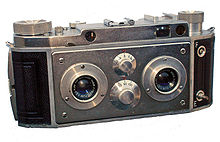
\includegraphics[width=\textwidth]{project/images/Verascope_40.jpg}
		\caption{\textsc{Verascope 40}}
		\label{fig:1}
	\end{subfigure}
	\hspace{3cm}
	\begin{subfigure}[b]{0.4\textwidth}
		\centering
		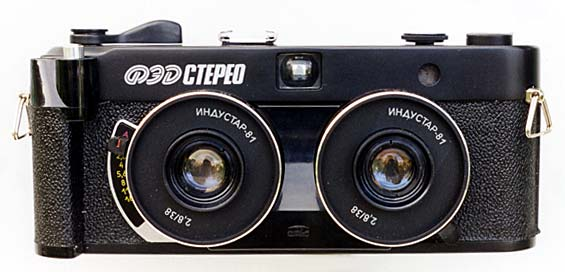
\includegraphics[width=\textwidth]{project/images/fedstereo.jpg}
		\caption{\textsc{FedStereo}}
		\label{fig:2}
	\end{subfigure}
	\caption{\textsc{Stereo Cameras}}
\end{figure}



